\documentclass[a4paper,12pt]{article}
\usepackage[left=2.5cm, right=2.5cm, top=2.5cm, bottom=2.5cm]{geometry}
\usepackage{pdfpages}
\usepackage{amssymb}
\usepackage{amsmath}
\usepackage{bm}
\usepackage{float}
\usepackage{csquotes}
\usepackage{subcaption}
\usepackage{booktabs}
\usepackage[
	style=authoryear,
	maxbibnames=100,
  natbib
]{biblatex}
\addbibresource{../bibliography.bib}

\DeclareBibliographyAlias{letter}{misc}

\setcounter{biburllcpenalty}{1}
\DeclareSortingTemplate{nymdt}{
  \sort{
    \field{presort}
  }
  \sort[final]{
    \field{sortkey}
  }
  \sort{
    \field{sortname}
    \field{author}
    \field{editor}
    \field{translator}
    \field{sorttitle}
    \field{title}
  }
  \sort{
    \field{sortyear}
    \field{year}
  }
  \sort{
    \field[padside=left,padwidth=2,padchar=0]{month}
    \literal{00}
  }
  \sort{
    \field[padside=left,padwidth=2,padchar=0]{day}
    \literal{00}
  }
  \sort{
    \field{sorttitle}
  }
  \sort{
    \field[padside=left,padwidth=4,padchar=0]{volume}
    \literal{0000}
  }
}

\usepackage{minted}
\setminted{frame=lines, fontsize=\small}
\usepackage{graphicx}
\usepackage{hyperref}
\hypersetup{
    colorlinks=true,
    linkcolor=black,
    filecolor=black,
    urlcolor=black,
    citecolor=black
}
\usepackage{algorithm}
\usepackage{algorithmic}
% Allow more flexible breaking of long URLs:
\setlength\emergencystretch{3em}
\setcounter{biburllcpenalty}{7000}
\setcounter{biburlucpenalty}{7000}
\Urlmuskip=0mu plus 1mu

\title{Distance-based dimensionality reduction for big data}
\author{Adrià Casanova Lloveras}

\begin{document}

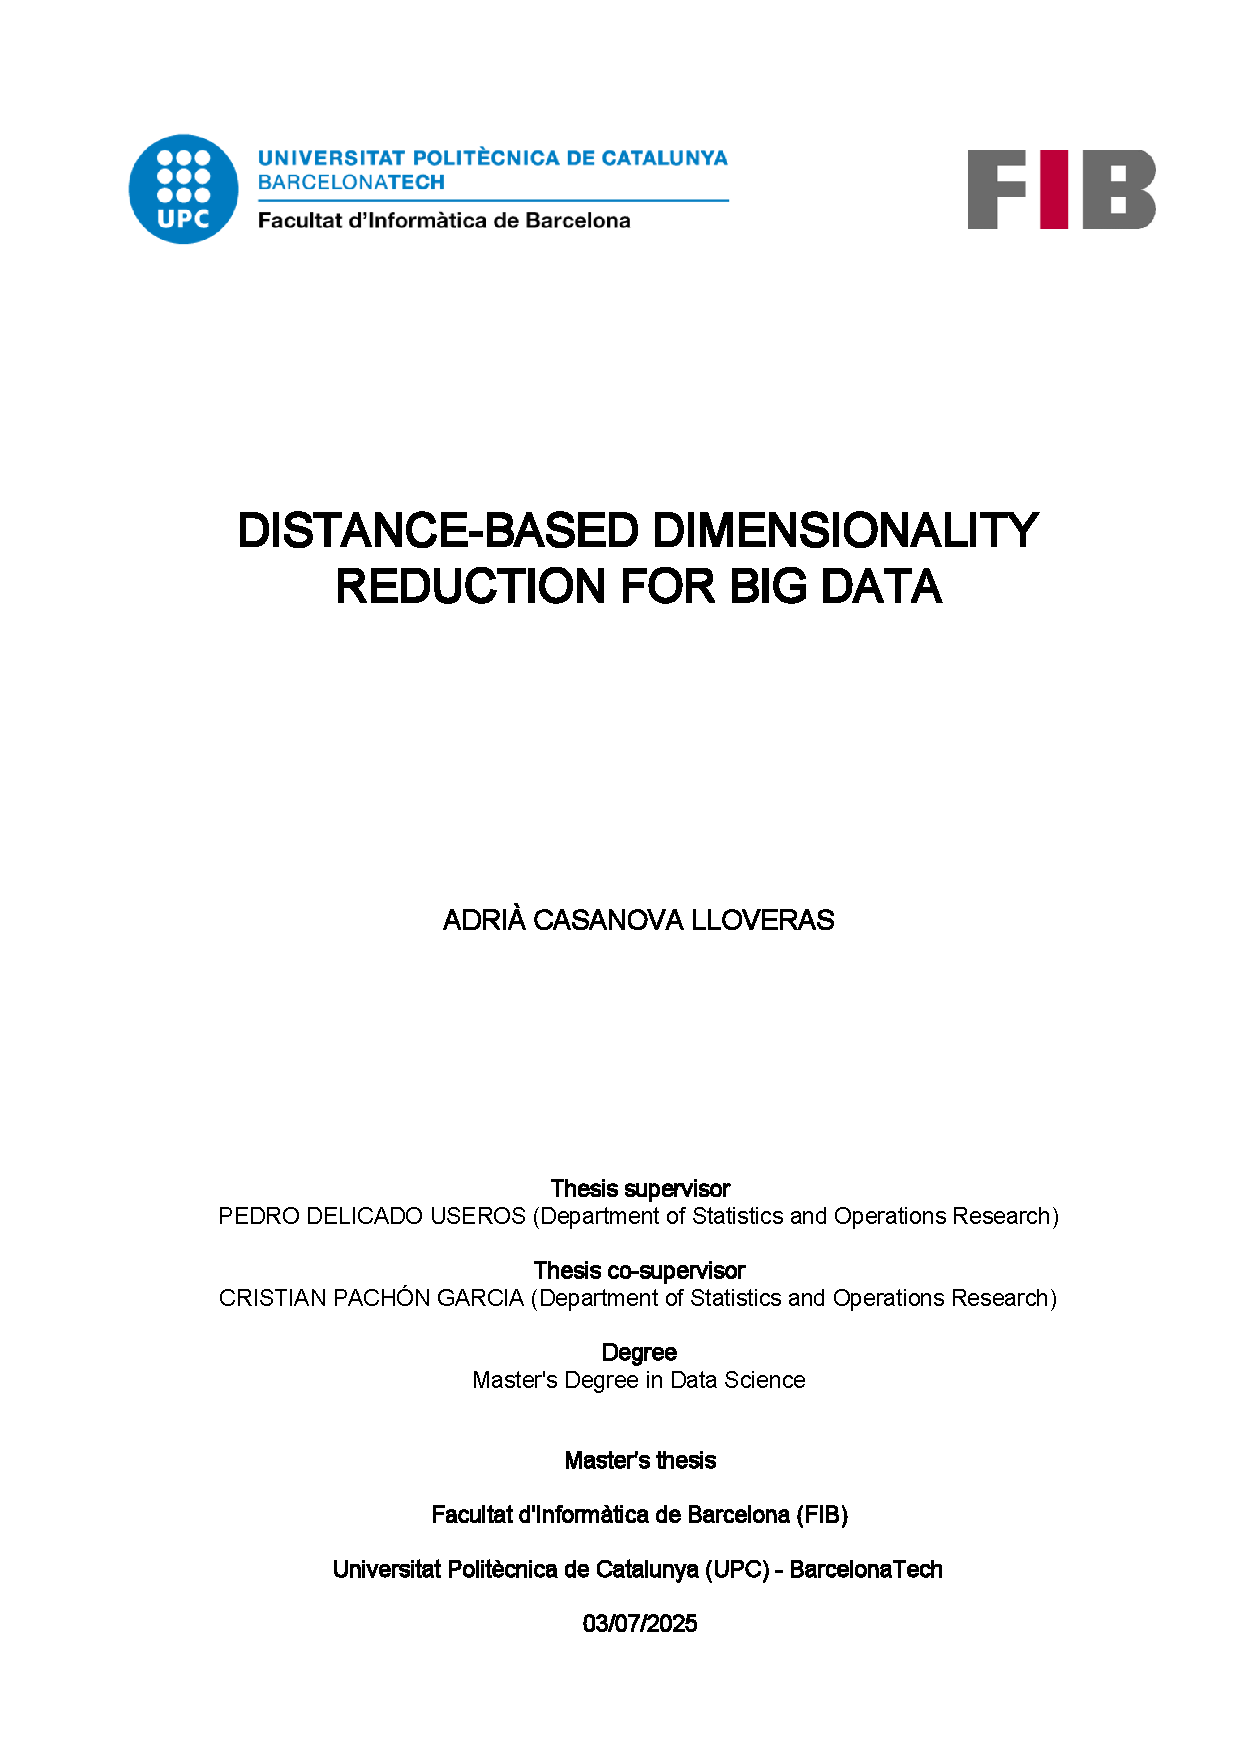
\includepdf{front_cover.pdf}

\section*{Acknowledgements}

Even though this master's thesis has been written in a small committee, I would like to appreciate the team my thesis supervisors and I have brought about during this semester. Our weekly video calls have become a space I will fondly remember for a long time. Thank you, Cristian and Pedro, for dedicating your time to help me bring forthward this project every week without fail. I have felt completely at ease under your supervision and you have given me the courage to overcome my recurring fears when I needed it most. I can confidently proclaim that your aid has been essential to bring this thesis to a success. Thank you.

\pagebreak
\begin{abstract}
    Dimensionality reduction aims to project a dataset into a low-dimensional space. Many techniques have been proposed, most of them based on the inter-individual distance matrix. When the number of individuals is really large, the use of full distance matrices is prohibitive because of their quadratic memory complexity. There are algorithms that extend classical multidimensional scaling (a long-established dimensionality reduction method based on distances) to the big data setting. In this TFM, we adapt these algorithms to any generic distance-based dimensionality reduction method.
\end{abstract}
\pagebreak

\tableofcontents
\pagebreak

\section{Introduction, Motivation, and Objectives}

\subsection{Introduction}

Dimensionality Reduction (DR) techniques embed high-dimensional datasets into signficantly lower-dimensional spaces while preserving the structure of the original data. Their primary goal is to tackle the common challegens of working with high-dimensional data, such as sparsity (caused by the curse of dimensionality) or large computational and storage costs.

That being said, DR is mainly used for visualization purposes. In this setting, complex high-dimensional data is projected into $\mathbb{R}^2$, making patters and clusters more apparent.

Many DR methods have been proposed since Principal Components Analysis (PCA) (the most famous linear method) was first introduced, each with distinct approaches and objectives. In particular, non-linear techniques have turned out to be very useful thanks to their ability to preserve complex relationships. Some examples are Multidimensional Scaling (MDS), Local MDS, Isomap, t-Distributed Stochastic Neighbor Embedding (t-SNE), Uniform Manifold Approximation and Projection (UMAP) and Autoencoder. All these methods differ in how they define and maintain relationships between points, although all try to preserve global structure and local neighborhoods.

Despite their utility, DR methods face a few limitations. Many algorithms require computing and/or keeping in memory pairwise distances between all data points, resulting in quadratic time complexity and memory requirements. This becomes prohibitive for large datasets with millions of points. Parameter selection presents challenges too, since there is no general consensus on the best way to tune them and $k$-fold cross ???? validation is very costly due to the substantial time complexities of these algorithms. Furthermore, information loss is inevitable during dimensionality reduction, and understanding which aspects of the data are preserved and which are distorted is crucial to correctly interpret the results.

\subsection{Motivation}

The recent advent of large data has led to new challenges and technologies to face them. When the number of observations of a dataset is very big, distance-based DR methods become computationally prohibitive because of their quadratic time and memory complexities. For example, working with a dataset of 100,000 individuals and 10 numeric variables would require a system with about 400GB of RAM.

Recently, \cite{Delicado2024} studied existing and new modifications of MDS to tackle big datasets, demonstrating significant improvements in computational efficiency while maintaining embedding quality. One of the variations they came up with followed a divide-and-conquer approach, that in principle could be generalized to any DR technique based on between-points distances.

\subsection{Objectives}

The primary goal of this thesis is to propose a divide-and-conquer framework for any generic distance-based dimensionality reduction method that effectively decreases the method's time and memory complexities. Specifically, we aim to:

\begin{enumerate}
    \item Review the literature to analyze the properties and applications of the most used DR techniques.
    \item Develop a generalized framework for distance-based DR methods that leverages the divide-and-conquer strategy and the Procrustes transformation to reduce time and memory complexities.
    \item Implement and parallelize the proposed framework for specific DR algorithms such as non-classical MDS, Local MDS, Isomap and t-SNE.
    \item Empirically evaluate the performance of the adapted algorithms in terms of computational efficiency, size limitations and quality of embeddings on benchmark datasets of varying sizes.
    \item Compare the results with the traditional counterpart of each tested DR method.
    \item Provide guidelines and best practices for selecting and tuning the proposed DR methods based on dataset characteristics and desired properties of the embedding.
\end{enumerate}

The successful completion of these objectives will contribute to making  dimensionality reduction techniques accessible for very large datasets, democratizing their use across scientific and industrial applications where data scale is a present challenge.
\pagebreak

\section{State of the art}

Many nonlinear DR techniques and big data solutions discovered in recent years have lead to our divide-and-conquer proposal. Hence, we shall first review them to understand the advances they have achieved. In section \ref{sec:DR-techniques}, our goal is to review four dimensionality reduction techniques that we will later apply our divide-and-conquer framework to. Next, in section \ref{sec:MDS-big-data}, we will showcase in more detail the work of \citet{Delicado2024} with respect to classical MDS in big data to motivate our choosing of the divide-and-conquer approach. Finally, sections \ref{sec:landmark-Isomap-OOC-DR-framework} and \ref{sec:openTSNE} offer a discussion about three more solutions to the big data problem in DR and how they relate to our proposal: landmark Isomap (\cite{Silva2002}), the out-of-core dimensionality reduction framework (\cite{Reichmann2024}) and novel Python t-SNE implementations.

\subsection{A few dimensionality reduction techniques}
\label{sec:DR-techniques}

\subsubsection{Non-classical MDS: the SMACOF algorithm}

SMACOF (Scaling by MAjorizing a COmplicated Function) is a multidimensional scaling procedure that minimizes metric stress using a majorization technique (\cite{Kruskal1964a,Kruskal1964b}). Given the distance matrix $\mathbf{D}_{\mathbf{X}} = (\delta_{ij})$ of the original high-dimensional data and its corresponding low-dimensional distance matrix $\mathbf{D}_{\mathbf{\tilde{Y}}} = (d_{ij})$, metric stress determines how much different $\mathbf{D}_{\mathbf{X}}$ and $\mathbf{D}_{\mathbf{\tilde{Y}}}$ are by the expression
$$
STRESS_M(\mathbf{D}_{\mathbf{X}}, \mathbf{D}_{\mathbf{\tilde{Y}}}) = \sqrt{\frac{\sum_{i<j}\left(\delta_{i j}-d_{i j}\right)^2}{\sum_{i<j} \delta_{i j}^2}}.
$$
SMACOF (see Algorithm \ref{alg:SMACOF}) is faster for this problem than general optimization methods, such as gradient descent, and it consists on iterative Guttman transformations \citep{Guttman1968} applied to the embedded data.

\begin{algorithm}[ht]
    \caption{SMACOF}
    \label{alg:SMACOF}
    
    \begin{algorithmic}[1]
    \REQUIRE $\mathbf{D}_{\boldsymbol{\mathbf{X}}} = (\delta_{ij})$, the $n\times n$ matrix of observed distances; $q$, the embedding's dimensionality; $n\_iter$, the maximum number of iterations; and $\varepsilon$, the convergence threshold.
    \ENSURE $\boldsymbol{\mathbf{\tilde{Y}}}$, a configuration in a $q$-dimensional space.
    \STATE Initialize at random $\boldsymbol{\mathbf{\tilde{Y}}}^{(0)} \in \mathbb{R}^{n \times q}$
    \STATE $k \leftarrow 0$
    \REPEAT
        \STATE Compute the distance matrix of $\boldsymbol{\mathbf{\tilde{Y}}}^{(k)}$, $\mathbf{D}_{\boldsymbol{\mathbf{\tilde{Y}}^{(k)}}}$, with entries $d_{ij}^k = \|\tilde{y}_i^{(k)} - \tilde{y}_j^{(k)}\|$
        \STATE Compute the metric stress: $STRESS_M( \mathbf{D}_{\mathbf{X}}, \mathbf{D}_{\boldsymbol{\mathbf{\tilde{Y}}^{(k)}}} )$
        \STATE Compute the Guttman transform: $\boldsymbol{\mathbf{\tilde{Y}}}^{(k+1)} = n^{-1}\mathbf{B}(\boldsymbol{\mathbf{\tilde{Y}}}^{(k)})\boldsymbol{\mathbf{\tilde{Y}}}^{(k)}$ where $\mathbf{B}(\boldsymbol{\mathbf{\tilde{Y}}}^{(k)}) = (b_{ij}^k)$:
        $$
        b_{ij}^k =
        \begin{cases}
        -\delta_{ij}/d_{ij}^k & \text{if } i \neq j \text{ and } d_{ij}^k > 0 \\
        0 & \text{if } i \neq j \text{ and } d_{ij}^k = 0 \\
        -\sum_{j \neq i} b_{ij}^k & \text{if } i = j
        \end{cases}
        $$
        \STATE $k \leftarrow k + 1$
    \UNTIL{$k \geq n\_iter$ or $|STRESS_M(D_{\mathbf{X}}, \boldsymbol{\mathbf{\tilde{Y}}}^{(k-1)}) - STRESS_M(D_{\mathbf{X}}, \boldsymbol{\mathbf{\tilde{Y}}}^{(k)}| < \varepsilon$}
    \RETURN $\boldsymbol{\mathbf{\tilde{Y}}}^{(k)}$
    \end{algorithmic}
\end{algorithm}

\subsubsection{Local MDS}

Local MDS \citep{Chen2009} is a variant of non-classical multidimensional scaling that differs in how large distances are treated. Specifically, a repulsive term between distant points is added to the stress function to further separate points in the low-dimensional configuration (see Algorithm \ref{alg:localMDS}). Parameters $\tau$ (which must be in the unit interval) and $k$ may be tuned with $k'$-cross validation thanks to the LC (Local Continuity) meta-criteria \citep{Chen2009}. (\textit{POSSIBLE ANNEX})

\begin{algorithm}[ht]
    \caption{Local MDS}
    \label{alg:localMDS}
    
    \begin{algorithmic}[1]
    \REQUIRE $\mathbf{D_X} = (\delta_{ij})$, the $n \times n$ matrix of observed distances; $q$, the embedding's dimensionality; $k$, the size of neighborhoods; and $\tau$, the weight of the repulsive term.
    \ENSURE $\mathbf{\tilde{Y}}$, a configuration in a $q$-dimensional space.
    \STATE Compute the symmetrized $k$-NN graph of $\mathbf{D_X}$, $\mathcal{N}_k$
    \STATE Calculate $t=\frac{|\mathcal{N}_k|}{\left|\mathcal{N}_k^C\right|} \cdot \operatorname{median}_{\mathcal{N}_k}\left(\delta_{ij}\right) \cdot \tau$
    \STATE Minimize the modified stress function:
    $$
    \mathbf{\tilde{Y}} = \min_{\mathbf{Y} \in \mathbb{R}^{n\times q}} \sum_{(i, j) \in \mathcal{N}_k}\left(\delta_{ij}-\left\|\mathbf{y}_i-\mathbf{y}_j\right\|\right)^2 - t \sum_{(i, j) \notin \mathcal{N}_k}\left\|\mathbf{y}_i-\mathbf{y}_j\right\|
    $$
    \RETURN $\mathbf{\tilde{Y}}$
    \end{algorithmic}
\end{algorithm}

\subsubsection{Isomap}

Isomap \citep{Tenenbaum2000} is a nonlinear technique that preserves geodesic distances between points in a manifold (see Algorithm \ref{alg:Isomap}). The key insight of Isomap is that large distances between objects are estimated from the shorter ones by the shortest path length. Then, shorter and estimated-larger distances have the same importance in a final classical MDS step.

The only tuning parameter of Isomap is the bandwidth, which can be interpreted as the limiting distance of nearest neighbors, $\varepsilon$,  or the amount of nearest neighbors per point, $k$. However, there is no consensus on what is the best method to choose it.

\begin{algorithm}[ht]
    \caption{Isomap}
    \label{alg:Isomap}

    \begin{algorithmic}[1]
    \REQUIRE $\mathbf{D_X}$, the $n \times n$ matrix of observed distances; $q$, the embedding's dimensionality; and $\varepsilon$, the limiting distance of nearest neighbors, or $k$, the amount of nearest neighbors per point.
    \ENSURE $\mathbf{\tilde{Y}}$, a configuration in a $q$-dimensional space.
    \STATE Find the $\varepsilon$-NN or $k$-NN graph of $\mathbf{D_X}$, $\mathcal{N}$
    \STATE Compute the distance matrix of $\mathcal{N}$, $\mathbf{D}_{\mathcal{N}}$
    \STATE Apply classical MDS to $\mathbf{D}_{\mathcal{N}}$: $\mathbf{\tilde{Y}} = \operatorname{MDS}(\mathbf{D}_{\mathcal{N}}, q)$
    \RETURN $\mathbf{\tilde{Y}}$
    
    \end{algorithmic}
\end{algorithm}

\subsubsection{t-SNE}

t-distributed stochastic neighbor embedding (t-SNE) is a nonlinear dimensionality reduction technique that preserves local neighborhoods by modeling similarities between points as conditional probabilities \citep{Vandermaaten2008}. The difference between these probability distributions in high and low-dimensional spaces is then minimized (see Algorithm \ref{alg:tSNE}).

t-SNE focuses on retaining the local structure of the data while ensuring that every point $\mathbf{y}_i$ in the low-dimensional space will have the same number of neighbors, making it particularly effective for visualizing clusters. The use of the Student's $t$ distribution with 1 degree of freedom (or Cauchy distribution) in the low-dimensional space addresses the \textit{crowding problem} by allowing dissimilar points to be modeled far apart (\cite{Vandermaaten2008}). The characteristic parameter of t-SNE is the perplexity, which can be interpreted as the average effective number of neighbors of the high-dimensional datapoints $\mathbf{x}_i$. Typical values are between 5 and 50.

\begin{algorithm}[ht]
    \caption{t-SNE}
    \label{alg:tSNE}
    
    \begin{algorithmic}[1]
    \REQUIRE $\mathbf{D_X} = (\delta_{ij})$, the $n \times n$ matrix of observed distances; $q$, the embedding's dimensionality; $Perp$, the perplexity.
    \ENSURE $\mathbf{\tilde{Y}}$, a configuration in a $q$-dimensional space.
    \STATE For every point $\mathbf{x}_i$, find $\sigma_i > 0$ so that the conditional probability ditribution
        $$
        p_{j|i} = \frac{\exp(-\delta_{ij}^2/2\sigma_i^2)}{\sum_{k \neq i}\exp(-\delta_{ik}^2/2\sigma_i^2)}\text{ if } i \neq j, \, p_{i|i} = 0
        $$ has perplexity $ Perp = 2^{-\sum_{j} p_{j|i} \log_2 p_{j|i}} $
    \STATE Symmetrize conditional distributions: $p_{ij} = \frac{p_{j|i} + p_{i|j}}{2n}$
    \STATE Consider Cauchy-distributed joint probabilities for the low-dimensional data $\mathbf{y}_i$: $$q_{ij} = \frac{(1 + \|y_i-y_j\|^2)^{-1}}{\sum_{h \neq k}(1 + \|y_h-y_k\|^2)^{-1}}$$
    \STATE Minimize the sum of Kullback-Leibler divergences between the joint distributions over all datapoints: $$
    \mathbf{\tilde{Y}} = \min_{\mathbf{Y} \in \mathbb{R}^{n\times q}} \sum_i \sum_j p_{j \mid i} \log \frac{p_{j \mid i}}{q_{j \mid i}}
    $$
    \RETURN $\mathbf{\tilde{Y}}$
    
    \end{algorithmic}
\end{algorithm}

\subsection{Multidimensional scaling for big data}
\label{sec:MDS-big-data}

\citet{Delicado2024} compared four existing versions of MDS with two newly proposed (divide-and-conquer MDS and interpolation MDS) to handle large datasets. As can be seen in Figure \ref{fig:bigmds}, these can be grouped into four categories:

\begin{itemize}
    \item \textbf{Interpolation-based}: landmark MDS, interpolation MDS and reduced MDS apply classical multidimensional scaling to a subset of $l \ll n$ points and then interpolate the projection of the remaining data. They differ in how the interpolation is computed: landmark MDS uses distance-based triangulation; interpolation MDS, the $l$-points Gower interpolation formula; and reduced MDS, the 1-point Gower interpolation formula.
    \item \textbf{Approximation-based}: pivot MDS approximates the SVD of the full inner product matrix with the SVD of the inner product matrix between a subset of $l \ll n$ points and all the points in the dataset.
    \item \textbf{Divide-and-conquer}: In divide-and-conquer MDS, the dataset is randomly partitioned into subsets of up to $l \ll n$ points into which MDS is independently applied. Then, the resulting embeddings are aligned with Procrustes transformations.
    \item \textbf{Recursive}: fast MDS is similar in spirit to divide-and-conquer MDS, but it partitions the data recursively. 
\end{itemize}

\begin{figure}[ht]
    \centering
    \captionsetup[subfigure]{labelformat=empty}

    \begin{subfigure}[t]{0.3\textwidth}
        \centering
        \includegraphics[width=.7\textwidth]{figures/landmark_MDS.png}
        \caption{landmark MDS}
        \label{fig:landmark_MDS}
    \end{subfigure}
    \hfill
    \begin{subfigure}[t]{0.3\textwidth}
        \centering
        \includegraphics[width=.7\textwidth]{figures/interpolation_adac.png}
        \caption{interpolation MDS}
        \label{fig:interpolation_MDS}
    \end{subfigure}
    \hfill
    \begin{subfigure}[t]{0.3\textwidth}
        \centering
        \includegraphics[width=.7\textwidth]{figures/reduced_MDS.png}
        \caption{reduced MDS}
        \label{fig:reduced_MDS}
    \end{subfigure}

    \begin{subfigure}[t]{0.3\textwidth}
        \centering
        \includegraphics[width=.7\textwidth]{figures/pivot_MDS.png}
        \caption{pivot MDS}
        \label{fig:pivot_MDS}
    \end{subfigure}
    \hfill
    \begin{subfigure}[t]{0.3\textwidth}
        \centering
        \includegraphics[width=.7\textwidth]{figures/divide_conquer_adac.png}
        \caption{divide-and-conquer MDS}
        \label{fig:divide_conquer_MDS}
    \end{subfigure}
    \hfill
    \begin{subfigure}[t]{0.3\textwidth}
        \centering
        \includegraphics[width=.9\textwidth]{figures/fast_adac.png}
        \caption{fast MDS}
        \label{fig:fast_MDS}
    \end{subfigure}
    
    \caption{Schematic representation of the six MDS algorithms for big data described in \cite{Delicado2024} (Source: original publication).}
    \label{fig:bigmds}
\end{figure}

\subsection{Landmark Isomap and the out-of-core dimensionality reduction framework}
\label{sec:landmark-Isomap-OOC-DR-framework}

\citet{Silva2002} first introduced landmark MDS as a step in landmark Isomap, a variation of Isomap that reduced the time complexity from $\mathcal{O}(n^3)$ to $\mathcal{O}(n^2l)$, where $l \ll n$ is the amount of landmark points. Other big data versions of MDS can be used with Isomap similarly. Nonetheless, interpolation-based and approximation-based algorithms cannot be trivially generalized to other nonlinear dimensionality reduction methods because they depend on the eigendecomposition computed in classical MDS.

Later, \citet{Reichmann2024} proposed the out-of-core dimensionality reduction framework. Similar to interpolation MDS, this algorithm applies a DR method that produces a mapping between high- and low-dimensional spaces (i.e. PCA, MDS, t-SNE, UMAP, autoencoders) to a small subset of the data and then projects the remaining datapoints in blocks. In order to obtain the aforementioned mappings, \citet{Reichmann2024} gathered a different projection mechanism for every method. PCA and autoencoders learn a parametric mapping between the original data and the embedding, so projecting new points is straightforward. For non-classical MDS, stress is minimized for a single point while keeping others fixed, a process known as \textit{single scaling} in the literature (\cite{Basalaj1999}). A similar strategy is used for t-SNE (\cite{Zhang2021}) and UMAP (\cite{McInnes2018a}), which leverage the k-NN of the projecting point to initialize the optimizer.

\subsection{openTSNE, an outstanding implementation of t-SNE}
\label{sec:openTSNE}

Maybe because of its popularity, t-SNE has been optimized for large data environments in Python through iterative implementations. \citet{Policar2024} considered many of them and published \verb|openTSNE|, a package that includes several t-SNE extensions \enquote{\textit{to address scalability issues and the quality of the resulting visualizations}}. Furthermore, they compared their proposal with those of other popular packages in serial and parallel configurations. In Figure \ref{fig:python_tsne_benchmarks} it can be seen that, thanks to these advances, the challenges of big data have already been solved in the specific case of t-SNE.

(\textit{POSSIBLE ANNEX})

\begin{figure}[ht]
    \centering
    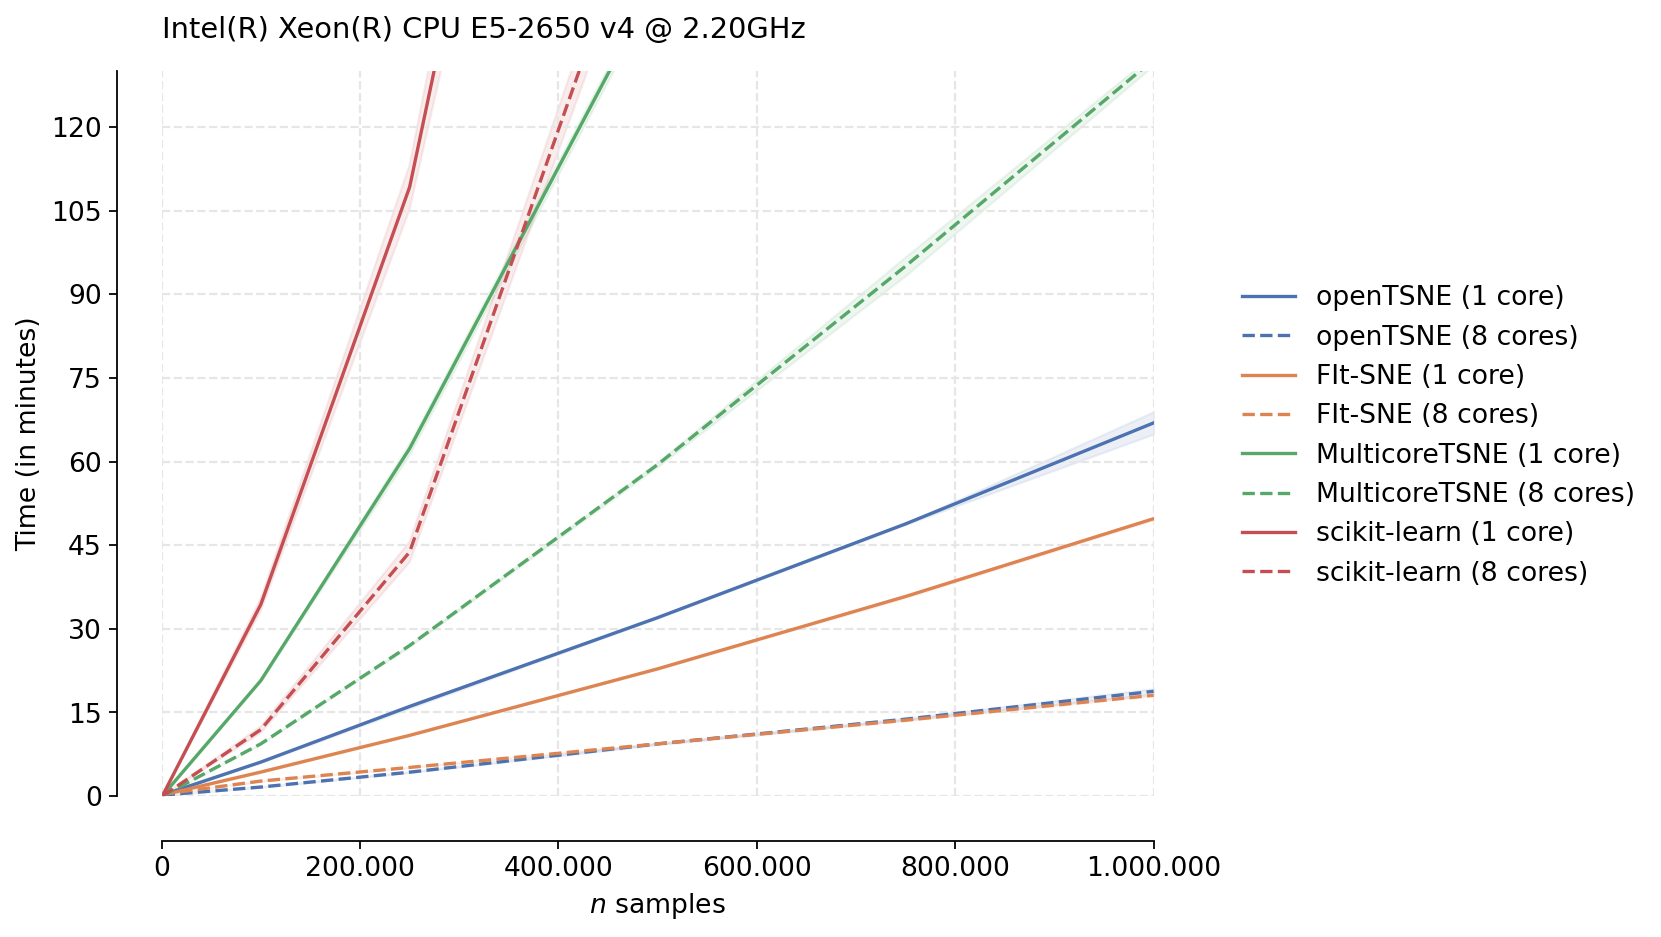
\includegraphics[width=0.8\textwidth]{figures/python_tsne_benchmarks.png}
    \caption{Benchmark of the best open-source t-SNE Python implementations by \cite{Poličar2023} (Source: original webpage).}
    \label{fig:python_tsne_benchmarks}
\end{figure}
\pagebreak

\section{Specification and design of the solution}
\label{sec:specification-and-design-of-the-solution}

Our solution to the problem of applying dimensionality reduction techniques to large datasets consists in dividing the data into partitions small enough for the computer to process and then merge their embeddings. As stated earlier, we follow the same approach as \citet{Delicado2024}. By means of an efficient alignment procedure named \textit{Procustes transformation}, we manage to orient every embedding to a specific alignment, with the goal that the final embedding will be coherent. Therefore, even though partitioning the data might modify the embedding's structure, our approach allows any system to tackle arbitrarily large datasets and leverage parallelization.

In order to preserve the geometry of the partition's embedding, we narrow Procustes transformations to rigid motions; that is, rotations and reflections. Moreover, we diminish the overhead computation of merging the embeddings by computing the transformation matrix with only a few datapoints. Specifically, if partitions have $l$ (or $l-1$) points, we sample $c < l$ from the first partition and stack them temporarily to every other partition. Later, we embed the first partition and extract the result of the $c$ sampled points, $\mathbf{\tilde{Y}}_{\mathcal{C}}$. Afterward, for every remaining partition, we project the stacked data with the chosen DR method and separate the $c$ points corresponding to the first partition, $\mathbf{\tilde{Y}}_{\mathcal{C}}^{(i)}$, from those of the current partition, $\mathbf{\tilde{Y}}_{i}$. This way, we can compute the optimal Procustes transformation between $\mathbf{\tilde{Y}}_{\mathcal{C}}$ and $\mathbf{\tilde{Y}}_{\mathcal{C}}^{(i)}$ and apply it to the larger matrix $\mathbf{\tilde{Y}}_i$, all without needing to process two full partitions.

For a more detailed specification of our solution, see Algorithm \ref{alg:DivideConquer}, which depicts the divide-and-conquer dimensionality reduction algorithm, and Section \ref{sec:Procrustes}, which shows how the Procrustes transformation can be obtained.

\begin{algorithm}
    \caption{Divide-and-conquer dimensionality reduction}
    \label{alg:DivideConquer}
    
    \begin{algorithmic}[1]
    \REQUIRE $\mathbf{D_X} = (\delta_{ij})$, the $n \times n$ matrix of observed distances; $\mathcal{M}$, the DR method; $l$, the partition size; $c$, the amount of connecting points; $q$, the embedding's dimensionality; and $arg$, $\mathcal{M}$'s specific parameters.
    \ENSURE $\mathbf{\tilde{Y}}$, a configuration in a $q$-dimensional space.
    
    \IF{$n \leq l$}
        \RETURN $\mathcal{M}(\mathbf{D_X}, q, arg)$
    \ENDIF
    
    \STATE Partition data into $k$ subsets: $\mathcal{P} = \{\mathcal{P}_1, \mathcal{P}_2, \ldots, \mathcal{P}_k\}$ where $|\mathcal{P}_i| \leq l$ for all $i$
    
    \STATE Sample $c$ connecting points from $\mathcal{P}_1$: $\mathcal{C} \subset \mathcal{P}_1$ with $|\mathcal{C}| = c$
    
    \STATE Apply DR method to first partition: $\mathbf{\tilde{Y}}_1 = \mathcal{M}(\mathbf{D_{X_{\mathcal{P}_1}}}, q, arg)$

    \STATE Extract embedding of $\mathcal{C}$: $\mathbf{\tilde{Y}}_\mathcal{C} = \mathbf{\tilde{Y}}_1[{\mathcal{C}},:]$
    
    \FOR{$i = 2$ to $k$}
        \STATE Stack connecting points to current partition: $\mathbf{X}_{\text{stack}} = [\mathbf{X}_{\mathcal{C}}; \mathbf{X}_{\mathcal{P}_i}]$
        \STATE Project stacked data: $\mathbf{\tilde{Y}}_{\text{stack}} = \mathcal{M}(\mathbf{D_{X_{\text{stack}}}}, q, arg)$
        \STATE Separate embedding of $\mathbf{X}_{\mathcal{C}}$: $\mathbf{\tilde{Y}}_{\mathcal{C}}^{(i)} = \mathbf{\tilde{Y}}_{\text{stack}}[1:c,:]$ and $\mathbf{\tilde{Y}}_i = \mathbf{\tilde{Y}}_{\text{stack}}[(c+1):,:]$
        \STATE Align projection using Procrustes: $\mathbf{\tilde{Y}}_i = \text{Procrustes}(\mathbf{\tilde{Y}}_\mathcal{C}, \mathbf{\tilde{Y}}_{\mathcal{C}}^{(i)}, \mathbf{\tilde{Y}}_i)$
    \ENDFOR
    
    \STATE Combine all projections: $\mathbf{\tilde{Y}}' = [\mathbf{\tilde{Y}}_1; \mathbf{\tilde{Y}}_2; \ldots; \mathbf{\tilde{Y}}_k]$
    \STATE Reorder rows to match original ordering: $\mathbf{\tilde{Y}}' = \mathbf{\tilde{Y}}'[\text{order},:]$
    \STATE Apply PCA to center and rotate for maximum variance: $\mathbf{\tilde{Y}}$ = PCA($\mathbf{\tilde{Y}}', q$)
    
    \RETURN $\mathbf{\tilde{Y}}$
    \end{algorithmic}
\end{algorithm}

\subsection{Orthogonal Procrustes transformation}
\label{sec:Procrustes}

Our problem of aligning the partitions' embeddings is known in the literature as the \textit{Procustes problem} (see, for instance, \citet{Borg2005}). Depending on the kind of fitting desired, different solutions can be found. For example, orthogonal transformations consist of rotations and reflections, but one may also desire dilations and shifts. In fact, the transformation could be any linear distortion.

That being said, in order to preserve the structure of every partitions' embedding and inter-individual distances, we considered best to limit the problem to rigid motions or, in other words, rotations and reflections. Now, let $\mathbf{A} \in \mathbb{R}^{c \times q}$ be the target configuration ($\mathbf{\tilde{Y}}_{\mathcal{C}}$ in Algorithm \ref{alg:DivideConquer}) and $\mathbf{B} \in \mathbb{R}^{c \times q}$ the corresponding testee ($\mathbf{\tilde{Y}}_{\mathcal{C}}^{(i)}$ in Algorithm \ref{alg:DivideConquer}). We wish to fit \textbf{B} to \textbf{A} by rigid motions. That is, we want to find the best orthogonal matrix \textbf{T} such that $\mathbf{A} \simeq \mathbf{BT}$.

To measure the $\simeq$ relation, we use the sum-of-squares criterion $L$. Then, the transformation $\mathbf{T}$ should be chosen to minimize $L$. Expressed in matrix notation, our problem is
$$
\min_{\mathbf{T} \in \text{O}(q)} L(\mathbf{T}) = \min_{\mathbf{T} \in \text{O}(q)} \text{tr}(\mathbf{A}-\mathbf{BT})(\mathbf{A}-\mathbf{BT})',
$$
where O($q$) is the orthogonal group in dimension $q$.

By expanding the expression of $L(\mathbf{T})$ and applying a lower bound inequality on traces derived by \citet{Kristof1970}, a global solution to the minimization problem can be found. Let $\mathbf{U}\boldsymbol{\Sigma}\mathbf{V}'$ be the singular value decomposition of $\mathbf{A}' \mathbf{B}$, where $\mathbf{U}' \mathbf{U}=\mathbf{I}, \mathbf{V}' \mathbf{V}=\mathbf{I}$, and $\boldsymbol{\Sigma}$ is the diagonal matrix with the singular values. Then, $L(\mathbf{T})$ is minimal if $\mathbf{T} = \mathbf{V} \mathbf{U}'$. Therefore, the Procrustes procedure we used would be as follows:

\begin{algorithm}
    \caption{Procrustes procedure}
    \label{alg:Procrustes}
    
    \begin{algorithmic}[1]
        \REQUIRE $\mathbf{A} \in \mathbb{R}^{c \times q}$, the target matrix; $\mathbf{B} \in \mathbb{R}^{c \times q}$, the testee matrix; and $\mathbf{C} \in \mathbb{R}^{m \times q}$, the matrix to transform.
        \ENSURE $\mathbf{C}'$, the matrix $\mathbf{C}$ after alignment.
        \STATE Multiply $\mathbf{M} = \mathbf{A}' \mathbf{B}$
        \STATE Compute singular value decomposition: $\mathbf{U}, \boldsymbol{\Sigma}, \mathbf{V}' = \text{SVD}(\mathbf{M})$
        \STATE Construct orthogonal matrix: $\mathbf{T} = \mathbf{V} \mathbf{U}'$
        \STATE Align $\mathbf{C}$: $\mathbf{C}' = \mathbf{CT}$
        \RETURN $\mathbf{C}'$
    \end{algorithmic}
\end{algorithm}
\pagebreak

\section{Development of the proposal}

\subsection{Python implementation of divide-and-conquer DR}
\label{sec:Python-implementation-of-divide-and-conquer-DR}

Given that R and Python are the standard programming languages in the data science field, we chose them as appropriate to implement the divide-and-conquer  DR algorithm. Initially, we aimed to develop and publish an R library because the thesis directors already had experience with the language. However, after reviewing the literature on DR for big data, we realized that many solutions were implemented in Python instead \citep{Reichmann2024}. So, in order to leverage the existing coding ecosystem, we switched to Python. From that moment onward, we documented the code development on an open-source GitHub repository (\href{https://github.com/airdac/TFM_Adria}{https://github.com/airdac/TFM\_Adria}). This system allowed us to easily update and share our implementations and experiments.

With time, the Python functions and classes we have written in different modules have become structured in a directory tree, hence taking the form of a package. Even though our project has not been published in any Python package index yet, it effectively works as a library. The main function is \verb|divide_conquer|, which implements Algorithm \ref{alg:DivideConquer} in parallel through the \verb|concurrent.futures| module. \verb|divide_conquer| also depends on private methods and requires a \verb|DRMethod| object as one of its arguments. This class, inherited from \verb|enum.Enum|, lists the supported DR methods in our package, which can be called through the \verb|get_method_function| method.

We have implemented and tested four DR algorithms: SMACOF, LMDS, Isomap and t-SNE, although adding more supported DR techniques in the future is straightforward because \verb|DRMethod| inherits from \verb|enum.Enum|. All but LMDS are wrappers to methods coded in other efficient and parallelized Python libraries. Specifically, we used the \verb|sklearn.manifold| module \citep{Pedregosa2011} for Isomap and SMACOF and \verb|openTSNE| \citep{Poličar2023} for t-SNE. LMDS, on the other hand, is a less popular method and, up to our knowledge, it has no public Python implementation at the moment. However, the R library \verb|smacofx| \citep{Leeuw2009} does, so we translated it to Python with the help of the \verb|scipy.spatial.distance| and \verb|sklearn.neighbors| modules. This also allowed us to optimize the LMDS runtime with the \verb|numba| just-in-time compiler \citep{Lam2015, Aycock2003}.

As shown in Section \ref{sec:experimentation-and-evaluation}, our implementation does not add a significant computation overhead when compared to standard DR techniques. In fact, divide-and-conquer DR leverages parallelization and provides a significant speed up to standard DR methods. Most DR techniques have quadratic time complexity \citep{Kruskal1964a,Kruskal1964b,Chen2009, Vandermaaten2008}, except for Isomap, whose computation time is cubic \citep{Tenenbaum2000}. Meanwhile, divide-and-conquer DR applies a DR method on $1 + \lceil \frac{n - l}{l - c} \rceil$ (which is about $n/l$ when $c \ll l$) partitions of $l$ or $l-1$ individuals and aligns them with orthogonal Procrustes transformations. Computing and applying one of these transformations takes three matrix multiplications and a singular value decomposition. Their time complexities, following the notation in Algorithm \ref{alg:Procrustes}, are $\mathcal{O}(cq^2)$ for $\mathbf{A}' \mathbf{B}$, $\mathcal{O}(q^3)$ for $\text{SVD}(\mathbf{M})$, $\mathcal{O}(q^3)$ for $\mathbf{V} \mathbf{U}'$ and $\mathcal{O}((l-c)q^2)$ for $\mathbf{CT}$. Therefore, the total time complexity of the Procustes procedure is $\mathcal{O}(q^2(l+q))$. Since it is computed for each partition but the first one and there are about $n/l$ of them when $c \ll l$, the resulting time complexity is approximately linear: $\mathcal{O}(n(l + q^2 + q^3/l))$ usually, but $\mathcal{O}(n(l^2 + q^2 + q^3/l))$ for Isomap. Note that reordering the rows in the low-dimensional configuration and applying PCA takes linear time.

The only DR method we have not been able to accelerate is t-SNE, given that it already was thouroughly optimized in the \verb|openTSNE| library \citep{Policar2024}. Finally, since we only keep in memory the inter-individual distance matrix of the partitions being embedded at each moment, our DR framework reduces space complexity from $\mathcal{O}(n^2)$ to $\mathcal{O}(l^2)$. That being said, the whole distance matrix (taking $\mathcal{O}(n^2)$ space) still needs to be stored in secondary memory.


\subsection{Experiments' methodology and parameter tuning}
\label{sec:experiment-methodology-parameter-tuning}

Once our framework was developed and we had implemented a few DR methods to test it, we run a series of experiments on the MNIST \citep{Cohen2017} and the Swiss roll \citep{Tenenbaum2000} datasets. On the one hand, we downloaded the MNIST dataset from the NIST webpage \citep{NIST2024}. On the other hand, we generated points on the Swiss roll manifold with the \verb|sklearn.datasets.make_swiss_roll| function \citep{Pedregosa2011}. All these experiments were executed, logged, plotted and discussed on Jupyter notebooks \citep{Kluyver2016} with the help of common Python packages such as \verb|numpy| \citep{Harris2020}, \verb|pandas| \citep{Mckinney2010}, \verb|matplotlib.pyplot| \citep{Hunter2007} or \verb|logging|. Furthermore, results were serialized with the \verb|pickle| module in final tests.

The MNIST dataset consisted of 345,035 pictures of hand-drawn digits represented in $\mathbb{R}^{784}$. Each dimension would correspond to the intensity of a pixel in grayscale and there were $28 \times 28$ of them. See Figure \ref{fig:MNIST} to observe a few pictures in the dataset. On the other hand, the Swiss roll dataset was sampled from a bidimensional object in $\mathbb{R}^3$ (see Figure \ref{fig:swiss-roll}) shaped like a sheet of paper curved into a spiral along its longest axis. In order to measure the time complexity of divide-and-conquer DR, we randomly generated datasets with sizes ranging between $10^3$ and $10^8$ points. A good embedding of the Swiss roll into $\mathbb{R}^2$ should intuitively be a rectangle, as if the Swiss roll were unfolded. In MNIST, we would like to obtain 10 clearly distinct clusters corresponding to each digit present in the dataset.

\begin{figure}
    \centering
    \includegraphics[width=0.5\textwidth]{figures/swiss-roll.png}
    \caption{The Swiss roll manifold. Color represents the angle of rotation along the spiral.}
    \label{fig:swiss-roll}
\end{figure}

\begin{figure}
    \centering
    \includegraphics[width=0.5\textwidth]{figures/MNIST.png}
    \caption{Four sampled images of the MNIST dataset.}
    \label{fig:MNIST}
\end{figure}

The general experimental methodology we used consisted in a series of steps. Given that working with big datasets is costly, we randomly sampled a subset of 1000 points and embedded it into $\mathbb{R}^2$ with a traditional DR technique. To distinguish it from its divide-and-conquer version, we called it a \textit{bare} technique. Then, before increasing the size of the dataset, we tuned the parameters of the method by applying it to the same dataset with different value combinations. In the tuning process, we took into account the runtime and embedding quality for each value combination. Our goal was to find parameter values that provided a good trade-off between speed and preserving the structure of the data. In Section \ref{sec:experimentation-and-evaluation}, we enter into more detail on the qualitative assessment of each dataset's embeddings.

Once parameters were tuned with a small enough subset of the data for our system to handle, we applied divide-and-conquer DR to larger datasets with partitions of $l=1000$ points. In comparison, when we applied the bare techniques to big datasets, execution would crash because of a lack of main memory. Hence, as shown in Section \ref{sec:experimentation-and-evaluation}, we managed to extend the functionality of DR techniques to arbitrarily large datasets.
\pagebreak

\section{Experimentation and evaluation of the proposal}
\label{sec:experimentation-and-evaluation}

The goal of this section is to present the experiments we have conducted on the divide-and-conquer DR algorithm to assess its quality and performance. Following the methodology described in section \ref{sec:experiment-methodology-parameter-tuning}, we were able to corroborate the space and time complexity of the procedure and understand better it's embedding mechanism. We chose the swiss roll and MNIST datasets for the tests because of their popularity, which makes it easier to compare our method with others in the literature, and because of how well Isomap and t-SNE embedded them. That allowed us to go even further and succesfully unfold a $10^8$ points swiss roll with divide-and-conquer Isomap. On the other hand, the classification task in the MNIST dataset proved more complicated to our algorithm, which was slower and separated digits worse than \verb|openTSNE|'s implementation of t-SNE.

The experimentation and evaluation process also provided us some insights on the standard SMACOF, LMDS, Isomap and t-SNE techniques. For example, we realized that LMDS, a nonlinear method intended to overcome the limitations of the SMACOF algorithm \citep{Chen2009}, was not able to unfold the swiss roll dataset. Even after having tuned the $k$ and $\tau$ parameters (see Algorithm \ref{alg:LMDS}), its embedding was porous and irregular instead of uniform and rectangular (see Figure \ref{fig:LMDS-swiss-roll}). Further research on this problem might lead to the development of a variation of LMDS that reduces the dimensionality of the swiss roll better.

Finally, we will describe the computer system we perfomed the tests on. Even though our main development computer was a  Macbook Pro (14-inc, Nov 2023) with 16 GB of RAM and the Apple M3 chip, we noticed that the \verb|concurrent.futures| module, which parallelized the execution of Algorithm \ref{alg:DivideConquer}, did not work in Mac computers with ARM chipsets. Therefore, we ended up using a Windows system. Specifically, our PC was an Asus ROG G513QM-HF026 laptop with the AMD Ryzen 7 5800H CPU, 16 GB of DDR4-3200MHz RAM, an SSD M.2 NVMe PCIe 3.0 and an NVIDIA RTX 3060 GPU.

\subsection{Initial runtime benchmarks}

Isomap was the first DR method we implemented into our divide-and-conquer framework, so it also was the first method we benchmarked. We tested divide-and-conquer Isomap on the swiss roll dataset with different parameter combinations and with parallel and serial computation. However, in all tests the number of connecting points for the Procrustes transformation was 100. We chose this number because, based on the thesis directors' experience on big data MDS \citep{Delicado2024}, it guaranteed good links between partitions' embeddings and efficient computations when $1,000 \leq l \leq 10,000$. Figure \ref{fig:Isomap-benchmark} shows the average runtimes of 20 experiments with different sets of parameters and dataset sizes. Parameters were previously tuned to ensure embeddings would preserve the structure of the data. As described in section \ref{sec:experiment-methodology-parameter-tuning}, we applied bare Isomap to swiss rolls of 1,000, 3,162 and 10,000 points, following a logarithmic sequence. Notice that we increased the number of neighbors $k$ for larger values of $l$ because partitions were denser.

After some experimentatiton, we realized that if $l=3162$ and $k=10$, the embedding was nearly perfect no matter the amount of individuals (see Figure \ref{fig:Isomap-huge}). Meanwhile, when $l=10,000$ and $k=15$, quality was similar and time was significantly larger, so we used $l=3162$ and $k=10$ for the largest datasets. This way, we managed to embed $10^8$ three-dimensional points into the Euclidean plane in about 3 hours. Hence, we showed that divide-and-conquer Isomap is capable of handling arbitrarily large datasets on a standard computer while maintaining the quality of the embedding.

Regarding parallelization, we can observe in Figure \ref{fig:Isomap-benchmark} that it effectively reduces the time complexity of divide-and-conquer DR, although its overhead slows down the algorithm when $n \leq 10^4$. Overall, results show that divide-and-conquer Isomap is linear in time with respect to $n$.

\begin{figure}[ht]
    \centering
    \includegraphics[width=0.8\textwidth]{figures/Isomap-benchmark.png}
    \caption{Runtime (s) of divide-and-conquer Isomap averaged over 20 experiments. Tests were performed on datasets generated on the swiss roll manifold \citep{Spiwokv2007} with sizes ranging from $10^3$ to $10^8$. Data was embedded into $\mathbb{R}^2$ with different parameter combinations and $c=100$. Runtime in parallel and serial execution is also compared.}
    \label{fig:Isomap-benchmark}
\end{figure}

\begin{figure}[ht]
    \centering
    \includegraphics[width=0.8\textwidth]{figures/Isomap-huge.png}
    \caption{Bidimensional embedding of a $10^8$ points swiss roll dataset \citep{Spiwokv2007} computed by divide-and-conquer Isomap with $l=3,162, \, c=100$ and $k=10$. Color represents the angle of rotation along the swiss roll spiral.}
    \label{fig:Isomap-huge}
\end{figure}

Afterwards, we tested divide-and-conquer t-SNE on the same datasets (see Figure \ref{fig:t-SNE-benchmark}). However, t-SNE performed notably slower than Isomap on the swiss roll, so we only run its divide-and-conquer variation with one parameter combination, $c = 100, \, l=1,000, \, Perp=30, \, n\_iter=250$. $n\_iter$ is the number of iterations carried out to minimize the Kullback-Leibler divergence \citep{Kullback1951}.

Even though divide-and-conquer t-SNE is about two orders of magnitud slower than divide-and-conquer Isomap, time complexity is linear as well, proving the expected results. The quality of the embedding, on the other hand, is very low. See Figure \ref{fig:t-SNE-huge} to observe that the structure of the data is broken into separate parts and the spiral shape is not unfolded.

\begin{figure}[ht]
    \centering
    \includegraphics[width=0.8\textwidth]{figures/tSNE-benchmark.png}
    \caption{Runtime (s) of divide-and-conquer Isomap and divide-and-conquer t-SNE averaged over 20 experiments. Tests were performed on datasets generated on the swiss roll manifold \citep{Spiwokv2007} with sizes ranging from $10^3$ to $10^8$. Data was embedded into $\mathbb{R}^2$ with different parameter combinations and $c=100$.}
    \label{fig:t-SNE-benchmark}
\end{figure}

\begin{figure}[ht]
    \centering
    \includegraphics[width=0.8\textwidth]{figures/t-SNE-swiss-roll-huge.png}
    \caption{Bidimensional embedding of a $10^6$ points swiss roll dataset \citep{Spiwokv2007} computed by divide-and-conquer t-SNE with $l=1,000, \, c=100, \, Perp=30$ and $n\_iter=250$. Color represents the angle of rotation along the swiss roll spiral.}
    \label{fig:t-SNE-huge}
\end{figure}

\subsection{Analysis of possible overheads in divide-and-conquer DR}

One reasonable question to formulate about the divide-and-conquer approach is whether splitting the data and merging the resulting embeddings constitue a significant computational cost in comparison to reducing each partition's dimensionality. Theoretically, fractionating the data should be rapid. As for the merging of partitions' embeddings, in section \ref{sec:specification-and-design-of-the-solution} we depicted how we align and overlap them with Procustes transformations between each embedding and one in specific (the first one). We intentionally find a rigid transformation only with a random subset of $c < l$ points to accelerate its computation, and then multiply the full partition's embedding with the $q\times q$ matrix of the transformation. Therefore, the overhead of merging embeddings should be insignificant.

Table \ref{tab:dc-overhead} shows the results of an experiment where each part of the divide-and-conquer DR algorithm was independently timed. We uniformly sampled 5,000 points from the MNIST dataset and embedded them into the Euclidean plane with divide-and-conquer SMACOF. The arguments used were $l=1000,\, c=100,\, n\_iter = 300,\, \varepsilon = 0.001$. As it was expected, neither partitioning the dataset nor aligning the partial embeddings entail a noteworthy overhead in divide-and-conquer DR. Indeed, the prior and the latter were about 5,506 times and 50,710 times swifter than embedding all partitions with SMACOF, respectively.

\begin{table}[ht]
    \centering
    \begin{tabular}{lccc}
        \toprule
        Operation    & Divide & Embed & Merge \\
        \midrule
        Duration (s) & $6.88 \times 10^{-3}$ & 37.9 & $7.47 \times 10^{-4}$ \\
        \bottomrule
    \end{tabular}
    \caption{Runtime (s) of each step of divide-and-conquer SMACOF on a 5000-point random subset of MNIST. The arguments used were $l=1000,\, c=100,\, n\_iter = 300,\, \varepsilon = 0.001$.}
    \label{tab:dc-overhead}
\end{table}

\subsection{Divide-and-conquer SMACOF}

\subsubsection{Swiss roll}

In this experiment, we applied bare and divide-and-conquer SMACOF to swiss rolls of different sizes. The largest dataset the standard method could handle ended up having 7,500 individuals and taking about 16 minutes to calculate. When we applied bare SMACOF to a 10,000 points swiss roll, the system crashed because it lacked main memory. Therefore, we show in Figure \ref{fig:SMACOF-swiss-roll-7500} the results of the test with 7,500 points.

The spiraled shape of both embeddings suggest that SMACOF cannot identify the intrinsic dimensionality of the swiss roll. Moreover, SMACOF condenses more the outer part of the manifold than the inner one and presents rugged edges. Regarding the qualitative differences between the bare and the divide-and-conquer versions, there is not much to be said. Divide-and-conquer SMACOF makes a good job aligning the partial configurations and obtains a similar embedding than bare SMACOF up to a 180º rotation.

To conclude, even though the SMACOF algorithm is not capable of properly embedding the swiss roll, we can see a clear advantage in using it on other datasets with the divide-and-conquer framework. Indeed, divide-and-conquer SMACOF is about 22 times faster than the bare method while returning a similar low-dimensional configuration.

\begin{figure}[ht]
    \centering
    \includegraphics[width=0.95\textwidth]{figures/SMACOF-swiss-roll-7500.png}
    \caption{Comparison of the bidimensional embeddings of a 7,500 points swiss roll dataset \citep{Spiwokv2007} by bare (left) and divide-and-conquer (right) SMACOF. The arguments used were $n\_iter = 300,\, \varepsilon = 0.001$ and in divide-and-conquer there also were $l=1000$ and $c=100$. Color represents the angle of rotation along the swiss roll spiral.}
    \label{fig:SMACOF-swiss-roll-7500}
\end{figure}


\subsubsection{MNIST}

Next, we try with a subpartition of 5000 images, since that worked properly with the swiss roll. We tried a few parameter combinations and obtained the best one for ... Figure \ref{fig:SMACOF-MNIST-kde} shows it is not bad, although 4, 7 and 9 are expectedly mixed. 5 could also be confused by 2 and 8 and viceversa. All normal here, their shapes are indeed similar.

Maybe I should talk about dimension correlation between SMACOF and divide-and-conquer SMACOF. The point of this is the framework, not the DR method, you know?

Total correlation of dim1: -0.8996107183598692
Total correlation of dim2: 0.8785425518794896

Merda, i falta el temps.

\begin{figure}[ht]
    \centering
    \includegraphics[width=0.95\textwidth]{figures/SMACOF-MNIST-kde.png}
    \caption{SMACOF-MNIST-kde}
    \label{fig:SMACOF-MNIST-kde}
\end{figure}

\begin{figure}[ht]
    \centering
    \includegraphics[width=0.95\textwidth]{figures/SMACOF-MNIST-coords.png}
    \caption{SMACOF-MNIST-coords}
    \label{fig:SMACOF-MNIST-coords}
\end{figure}

\begin{figure}[ht]
    \centering
    \includegraphics[width=0.8\textwidth]{figures/SMACOF-MNIST-huge.png}
    \caption{SMACOF-MNIST-huge}
    \label{fig:SMACOF-MNIST-huge}
\end{figure}

\subsection{Divide-and-conquer LMDS}

\subsubsection{Swiss roll}

Consider a swiss roll of 1,000 points. Well, LMDS makes trash out of it. Figure \ref{fig:LMDS-swiss-roll}.

\begin{figure}[ht]
    \centering
    \includegraphics[width=0.8\textwidth]{figures/LMDS-swiss-roll.png}
    \caption{LMDS devorant rollito de suís sionista, 1954.}
    \label{fig:LMDS-swiss-roll}
\end{figure}

\subsubsection{MNIST}

Same 5000 points MNIST subset, mate. Oh, but this is very bad... Like, worse than SMACOF HAHAHAHAHA.

Parla del temps i la correlació dimensionaaaaaaal.

Total correlation of dim1: 0.9489962757561992
Total correlation of dim2: -0.8206029210441554

\begin{figure}[ht]
    \centering
    \includegraphics[width=0.95\textwidth]{figures/LMDS-MNIST.png}
    \caption{L'LMDS es menja el 4.}
    \label{fig:LMDS-MNIST}
\end{figure}

\begin{figure}[ht]
    \centering
    \includegraphics[width=0.8\textwidth]{figures/LMDS-MNIST-huge.png}
    \caption{LMDS-MNIST-huge}
    \label{fig:LMDS-MNIST-huge}
\end{figure}

\subsection{Divide-and-conquer Isomap}

\subsubsection{Swiss roll}

Aaaaah... I don't have the same here. Gotta get those damn plots. Well we've seen this before, in the initial benchmark. Just go see Figure \ref{fig:Isomap-huge}.

\subsubsection{MNIST}

There you go, Figure \ref{fig:Isomap-MNIST}. It's just so bad HAHAHAHAHAH I can't handle this anymore.

Total correlation of dim1: 0.9195527127381181
Total correlation of dim2: -0.8623571714329816

\begin{figure}[ht]
    \centering
    \includegraphics[width=0.95\textwidth]{figures/Isomap-MNIST.png}
    \caption{Isomap, babyyyyyy.}
    \label{fig:Isomap-MNIST}
\end{figure}

\begin{figure}[ht]
    \centering
    \includegraphics[width=0.8\textwidth]{figures/Isomap-MNIST-huge.png}
    \caption{Isomap-MNIST-huge}
    \label{fig:Isomap-MNIST-huge}
\end{figure}

\subsection{Divide-and-conquer t-SNE}

\subsubsection{Swiss roll}

t-SNE is specially useful for visualization, so we will focus on MNIST. Nonetheless, here's the swiss roll. Figure \ref{fig:t-SNE-huge}.

\subsubsection{MNIST}

EXPLICAR EXEMPLE DUES PARTICIONS: LA QUALITAT POT SER DOLENTA PERQUÈ ELS CLUSTERS TENEN UNA TOPOLOGIA DIFERENT

Total correlation of dim1: 0.8170763484715383
Total correlation of dim2: 0.32817864544487557

\begin{figure}[ht]
    \centering
    \includegraphics[width=0.95\textwidth]{figures/t-SNE-MNIST-partitions.png}
    \caption{t-SNE on the numerets, germà gran.}
    \label{fig:t-SNE-MNIST-partitions}
\end{figure}

\begin{figure}[ht]
    \centering
    \includegraphics[width=0.95\textwidth]{figures/t-SNE-MNIST-5000.png}
    \caption{t-SNE on the numerets, germà gran.}
    \label{fig:t-SNE-MNIST}
\end{figure}

AAAAAAAAra bé, l'original no només és millor; també és més ràpid! Va, mira què passa quan busquem una combinació de paràmetres pel t-SNE que funcioni bé amb 1000 dibuixets de números. Figure \ref{fig:t-SNE-MNIST-dc}. Però és que mira el bare hahahahahahah Figure \ref{fig:t-SNE-MNIST-bare}.

\begin{figure}[ht]
    \centering
    \includegraphics[width=0.8\textwidth]{figures/t-SNE-MNIST-dc.png}
    \caption{t-SNE on the tots numerets, germà gran, i dividint i conquerint!}
    \label{fig:t-SNE-MNIST-dc}
\end{figure}

\begin{figure}[ht]
    \centering
    \includegraphics[width=0.8\textwidth]{figures/t-SNE-MNIST-bare.png}
    \caption{t-SNE on the tots numerets, germà gran, openTSNE!}
    \label{fig:t-SNE-MNIST-bare}
\end{figure}

Conclusió: no hem guanyat aquesta batalla perquè la competència és un F1 i el nostre és un turisme. Però oi que no t'emportaries un F1 a la muntanya? Aaaaah-mic!

I ja estaria, xd. Anem bé de pàgines, béeeeeeeee.
\pagebreak

\section{Analysis of sustainability and ethical implications}

\subsection{GHG emissions}

The rise of data collection, transfer and computation brought by big data has caused the construction and operation of a substantial amount of data centers around the world. This infrastructure consumes a lot of electricity and therefore is responsible for abundant greenhouse gas (GHG) emissions that cannot be neglected \citep{IEA2025, Brierley2023}. In order to cope with the current demand of AI and ML tools without creating too large of an impact on the environment, their energetic cost should be reduced as much as possible, mainly through algorithm innovation, decrease of data transfer and storage costs, and improvement of CPUs', GPUs' and TPUs' efficiency.

Our divide-and-conquer framework falls into the first category of energy reduction strategies by decreasing the runtime and required system capabilities to reduce the dimensionality of a big dataset. Indeed, the global warming potential of the GHG emitted when running a procedure on any given computer linearly depends on the time it takes to complete \citep{Lannelongue2021}. Therefore, our divide-and-conquer framework not only reduces the time complexity of DR but also its pollution complexity. Additionally, our framework makes DR less dependent on supercomputers (which contaminate throughout its construction, maintenance and operation) thanks to its low space complexity.

Concluding, even though there is still an environmental cost to consider in DR, given that it is not such a common task as prompting large language models or other neural networks, we are confident that our algorithm is currently sustainable and it does not pose a threat to the environment. Actually, using our algorithm instead of traditional DR methods would reduce the left carbon footprint.

\subsection{Visibility of small communities}

DR methods can emphasize biases present in the data. This happens because when projecting only a few coordinates of a dataset, small clusters can be left behind in the remaining, not projected, coordinates and do not show in the final embedding. Hence, small communities can become invisible.

However, our divide-and-conquer framework allows users to diminish the bias added by DR techniques by increasing the number of individuals embedded. Indeed, adding more individuals also means increasing the chance to represent small communities in the low-dimensional configuration of the data. So, by utilizing divide-and-conquer DR and providing more data, the resulting embedding can become more truthful to diverse realities than if bare DR techniques were used instead.

We refer to Figures \ref{fig:SMACOF-MNIST-kde} and \ref{fig:SMACOF-MNIST-huge} for an example of the above-mentioned pehonomenon. While bare SMACOF is only capable of embedding small subsets of the MNIST dataset, divide-and-conquer SMACOF effectively embeds the whole dataset. This results in bare SMACOF homogenizing the class of pictures of sevens and divide-and-conquer SMACOF detecting two distinct ways of handwriting sevens which were misrepresented in the sampled subset. As a matter of fact, the kernel density estimation of the configuration embedded by divide-and-conquer SMACOF shows two separate modes in the class of sevens. Had we considered a social dataset instead of MNIST, divide-and-conquer DR would have allowed us to reduce the dimensionality of the data without discriminating underrepresented communities. Thus, proving our framework useful in these scenarios.
\pagebreak

\section{Conclusions}
\pagebreak

\printbibliography
\pagebreak


\end{document}